%%%%%%%%%%%%%%%%%%%%%%%%%%%%%%%%%%%%%%%%%%%%%%%%%%%%%%%%%
%     Updated LaTeX Template for Bit-Plane Slicing Assignment     %
%%%%%%%%%%%%%%%%%%%%%%%%%%%%%%%%%%%%%%%%%%%%%%%%%%%%%%%%%

\documentclass{article}

% --- Preamble: Required packages ---
\usepackage[a4paper, margin=1in]{geometry} % For setting page margins
\usepackage{graphicx}                     % For including images
\usepackage{amsmath}                      % For math equations
\usepackage{listings}                     % For formatting code
\usepackage{xcolor}                       % For custom colors in code
\usepackage{hyperref}                     % For clickable links and better navigation
\usepackage{float}                        % To hold figures in place with [H]

% --- Document Information ---
\title{Demonstration of Bit-Plane Slicing and Image Reconstruction}
\author{Your Name \\ Your Student ID}
\date{\today}

% --- Code Listing Style ---
\definecolor{codegreen}{rgb}{0,0.6,0}
\definecolor{codegray}{rgb}{0.5,0.5,0.5}
\definecolor{codepurple}{rgb}{0.58,0,0.82}
\definecolor{backcolour}{rgb}{0.95,0.95,0.92}

\lstdefinestyle{mystyle}{
    backgroundcolor=\color{backcolour},   
    commentstyle=\color{codegreen},
    keywordstyle=\color{magenta},
    numberstyle=\tiny\color{codegray},
    stringstyle=\color{codepurple},
    basicstyle=\footnotesize\ttfamily,
    breakatwhitespace=false,         
    breaklines=true,                 
    captionpos=b,                    
    keepspaces=true,                 
    numbers=left,                    
    numbersep=5pt,                  
    showspaces=false,                
    showstringspaces=false,
    showtabs=false,                  
    tabsize=2,
    classoffset=1, % Enable keywords for type hints
    morekeywords={np, cv2, Path, List},
    keywordstyle=\color{blue},
    classoffset=0,
}
\lstset{style=mystyle}

% --- Start of Document ---
\begin{document}

\maketitle
\thispagestyle{empty}
\newpage

\tableofcontents
\newpage

% --- Section 1: Introduction and Theory ---
\section{Introduction to Bit-Plane Slicing}

Bit-plane slicing is a technique in digital image processing used to decompose a grayscale image into a series of binary images. For an 8-bit grayscale image, each pixel has an intensity value between 0 and 255. This value can be represented by an 8-bit binary number. Bit-plane slicing separates the image into 8 individual planes, where each plane corresponds to a specific bit position in the binary representation of the pixel values.

The intensity value $P$ of a pixel can be expressed as:
$$ P = \sum_{i=0}^{7} b_i \cdot 2^i = b_7 \cdot 2^7 + b_6 \cdot 2^6 + \dots + b_1 \cdot 2^1 + b_0 \cdot 2^0 $$
Where $b_i$ is the binary bit (0 or 1) at position $i$.

\begin{itemize}
    \item \textbf{Most Significant Bit (MSB):} The plane corresponding to the highest bit ($b_7$) is the MSB plane. It contains the most significant visual information and provides a rough approximation of the original image.
    \item \textbf{Least Significant Bit (LSB):} The plane corresponding to the lowest bit ($b_0$) is the LSB plane. It contains the finest details and is often where noise is most prominent.
\end{itemize}

This technique is useful for image compression, watermarking (by modifying the LSB plane), and understanding the contribution of each bit to the overall appearance of an image.

% --- Section 2: Python Implementation ---
\section{Python Implementation}
The following refactored Python script was used to perform the bit-plane slicing, progressive image reconstruction, and video generation. It utilizes libraries such as OpenCV, NumPy, and Matplotlib, with a focus on clarity, modularity, and modern coding practices.

\begin{lstlisting}[language=Python, caption={Rewritten Python script for bit-plane slicing and reconstruction.}, label={lst:code}]
# -*- coding: utf-8 -*-
"""
Demonstrates bit-plane slicing and progressive image reconstruction.

This script performs the following actions:
1. Loads a grayscale image or creates a sample one if not found.
2. Decomposes the image into its 8 constituent bit planes.
3. Saves each bit plane as an individual image.
4. Progressively reconstructs the image by adding bit planes from MSB to LSB.
5. Saves an image at each step of the reconstruction.
6. Generates a video showing the gradual improvement in image quality.
7. Creates summary images comparing all bit planes and reconstruction steps.
"""

import cv2
import numpy as np
import matplotlib.pyplot as plt
from pathlib import Path
from typing import List

# --- Configuration Constants ---
SOURCE_IMAGE_PATH = Path("image.png")
OUTPUT_DIR = Path("images")
VIDEO_FILENAME = "bit_plane_progression.mp4"
VIDEO_FPS = 1
FRAME_DURATION_SECONDS = 2

# --- Core Image Processing Functions ---

def extract_bit_plane(image: np.ndarray, bit_position: int) -> np.ndarray:
    """Extracts a specific bit plane from an 8-bit grayscale image."""
    mask = 1 << bit_position
    bit_plane = (image & mask) >> bit_position
    return (bit_plane * 255).astype(np.uint8)

def reconstruct_from_bit_planes(bit_planes: List[np.ndarray]) -> np.ndarray:
    """Reconstructs an image from a list of bit planes (MSB to LSB)."""
    reconstructed_image = np.zeros_like(bit_planes[0], dtype=np.uint8)
    for i, plane in enumerate(bit_planes):
        weight = 2 ** (7 - i)
        reconstructed_image += (plane // 255) * weight
    return reconstructed_image

# --- Helper & Utility Functions ---

def load_or_create_image(image_path: Path) -> np.ndarray:
    """Loads a grayscale image or creates a sample if not found."""
    if image_path.exists():
        return cv2.imread(str(image_path), cv2.IMREAD_GRAYSCALE)
    else:
        print(f"Image not found. Creating sample and saving to '{image_path}'")
        img = np.zeros((512, 512), dtype=np.uint8)
        cv2.rectangle(img, (50, 50), (200, 200), 128, -1)
        cv2.circle(img, (350, 256), 100, 220, -1)
        for i in range(512):
            img[i, :] = np.clip(img[i, :] + (i / 4), 0, 255)
        cv2.imwrite(str(image_path), img)
        return img

def add_text_overlay(image: np.ndarray, text: str) -> np.ndarray:
    """Adds a descriptive text overlay to an image."""
    output_image = cv2.cvtColor(image, cv2.COLOR_GRAY2BGR)
    cv2.rectangle(output_image, (0, 0), (output_image.shape[1], 40), (0, 0, 0), -1)
    cv2.putText(output_image, text, (10, 28), cv2.FONT_HERSHEY_SIMPLEX, 0.8, (0, 255, 0), 2)
    return output_image

# --- Main Application ---
def main():
    """Main function to run the entire bit-plane analysis process."""
    print("Starting Bit-Plane Slicing Demonstration...")
    OUTPUT_DIR.mkdir(exist_ok=True)
    original_image = load_or_create_image(SOURCE_IMAGE_PATH)
    cv2.imwrite(str(OUTPUT_DIR / "original_image.png"), original_image)

    all_bit_planes = [extract_bit_plane(original_image, i) for i in range(7, -1, -1)]
    for i, plane in enumerate(all_bit_planes):
        cv2.imwrite(str(OUTPUT_DIR / f"bit_plane_{7-i}.png"), plane)

    reconstructed_images = []
    video_frames = []
    for i in range(1, 9):
        planes_to_use = all_bit_planes[:i]
        reconstructed = reconstruct_from_bit_planes(planes_to_use)
        reconstructed_images.append(reconstructed)
        cv2.imwrite(str(OUTPUT_DIR / f"reconstructed_step_{i}.png"), reconstructed)
        
        bit_names = ", ".join([str(j) for j in range(7, 7 - i, -1)])
        info_text = f"Step {i}/8: Using Bits [{bit_names}]"
        video_frames.append(add_text_overlay(reconstructed, info_text))
        
    height, width, _ = video_frames[0].shape
    fourcc = cv2.VideoWriter_fourcc(*'mp4v')
    video_writer = cv2.VideoWriter(str(VIDEO_FILENAME), fourcc, VIDEO_FPS, (width, height))
    for frame in video_frames:
        for _ in range(FRAME_DURATION_SECONDS * VIDEO_FPS):
            video_writer.write(frame)
    video_writer.release()

if __name__ == "__main__":
    main()
\end{lstlisting}

% --- Section 3: Results and Analysis ---
\section{Results and Analysis}

\subsection{Original Image and Individual Bit Planes}
The process begins with a grayscale source image. This image is then decomposed into its eight constituent bit planes, from the Most Significant Bit (MSB, Bit 7) to the Least Significant Bit (LSB, Bit 0).

\begin{figure}[H]
    \centering
    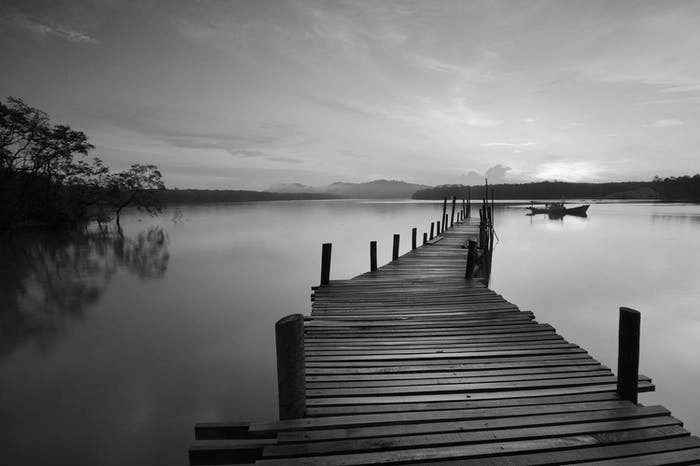
\includegraphics[width=0.4\textwidth]{images/original_image.png}
    \caption{The original grayscale image used for the demonstration.}
    \label{fig:original}
\end{figure}

\begin{figure}[H]
    \centering
    \begin{tabular}{ccc}
        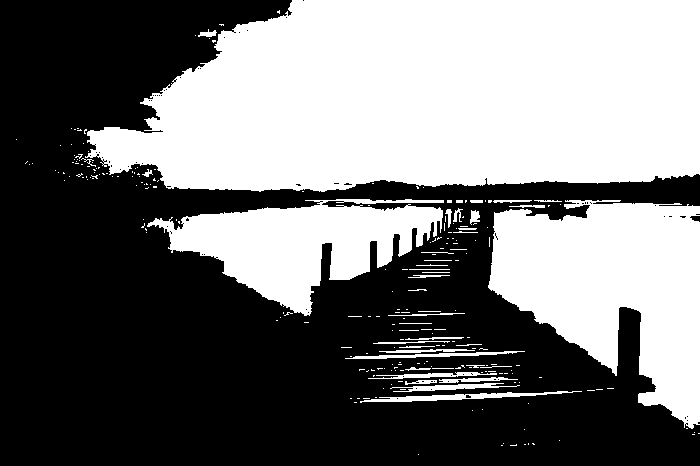
\includegraphics[width=0.3\textwidth]{images/bit_plane_7.png} &
        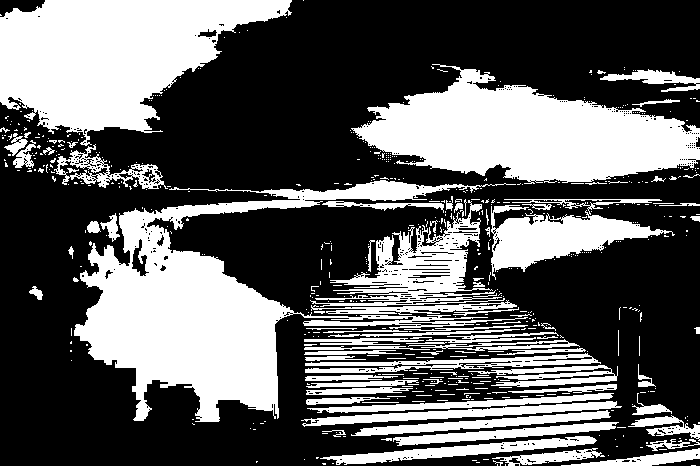
\includegraphics[width=0.3\textwidth]{images/bit_plane_6.png} &
        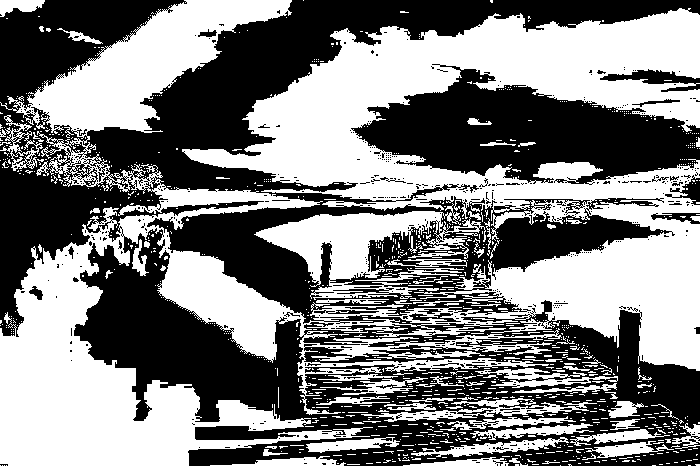
\includegraphics[width=0.3\textwidth]{images/bit_plane_5.png} \\
        Bit Plane 7 (MSB) & Bit Plane 6 & Bit Plane 5 \\
        \\
        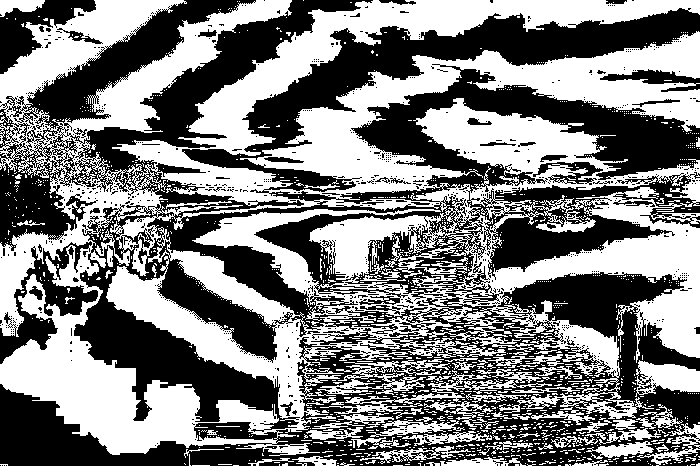
\includegraphics[width=0.3\textwidth]{images/bit_plane_4.png} &
        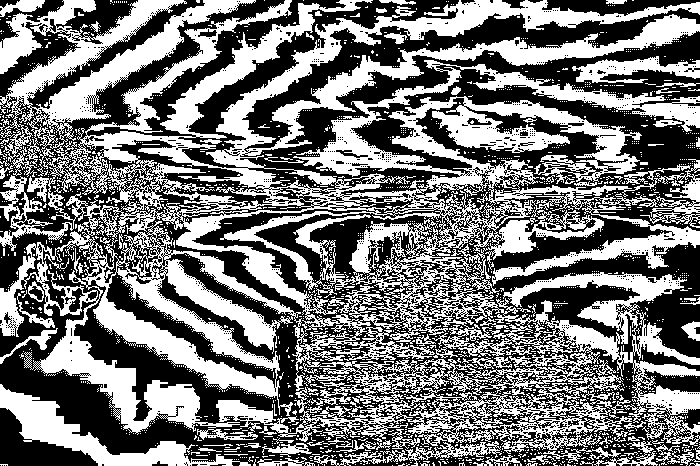
\includegraphics[width=0.3\textwidth]{images/bit_plane_3.png} &
        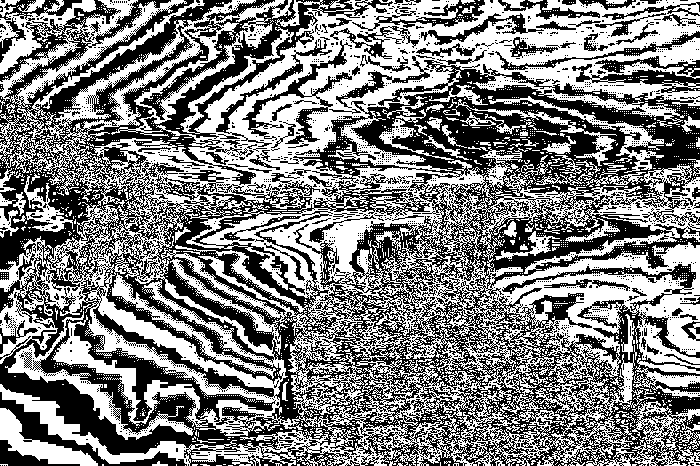
\includegraphics[width=0.3\textwidth]{images/bit_plane_2.png} \\
        Bit Plane 4 & Bit Plane 3 & Bit Plane 2 \\
        \\
        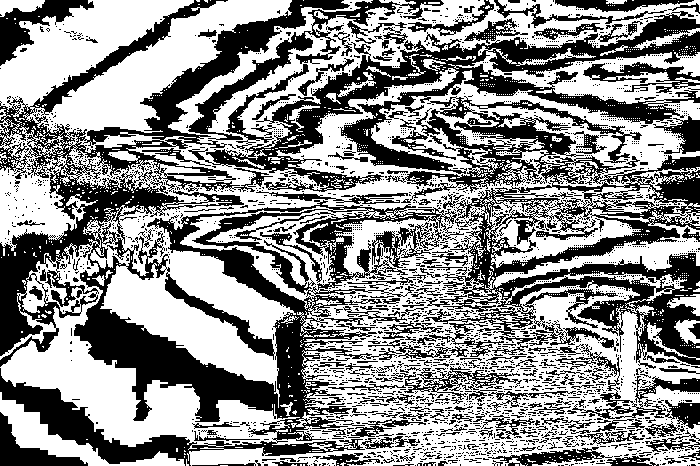
\includegraphics[width=0.3\textwidth]{images/bit_plane_1.png} &
        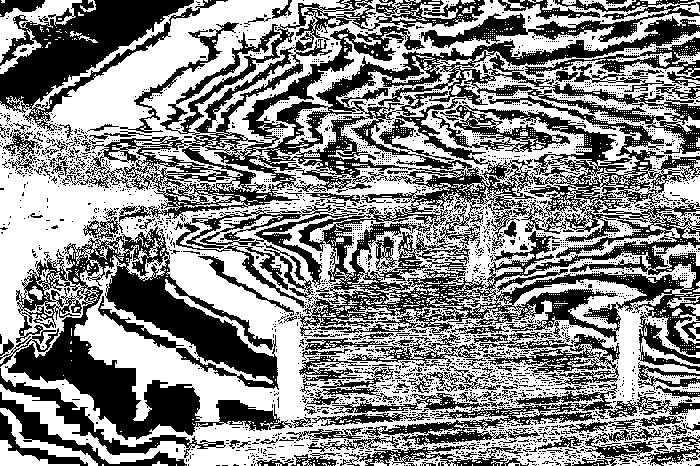
\includegraphics[width=0.3\textwidth]{images/bit_plane_0.png} &
        \\
        Bit Plane 1 & Bit Plane 0 (LSB) & \\
    \end{tabular}
    \caption{The eight individual bit planes extracted from the original image.}
    \label{fig:bitplanes}
\end{figure}

\clearpage
\subsection{Progressive Image Reconstruction}
The image is reconstructed progressively by adding one bit plane at a time, starting from the MSB (Bit 7). The visual quality of the reconstructed image improves with each added plane.

\begin{figure}[H]
    \centering
    \begin{tabular}{cc}
        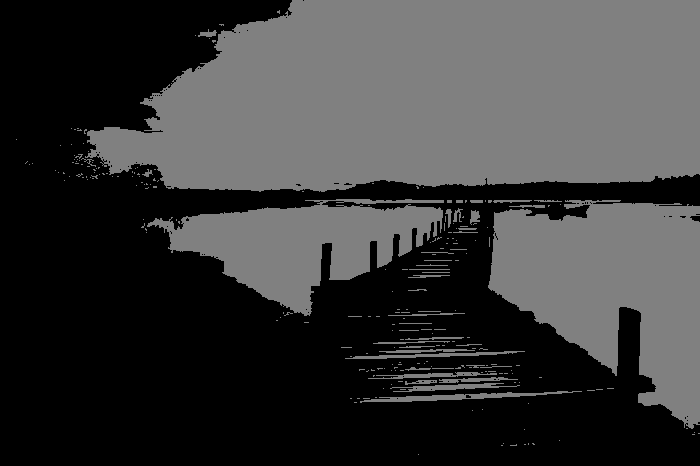
\includegraphics[width=0.4\textwidth]{images/reconstructed_step_1.png} &
        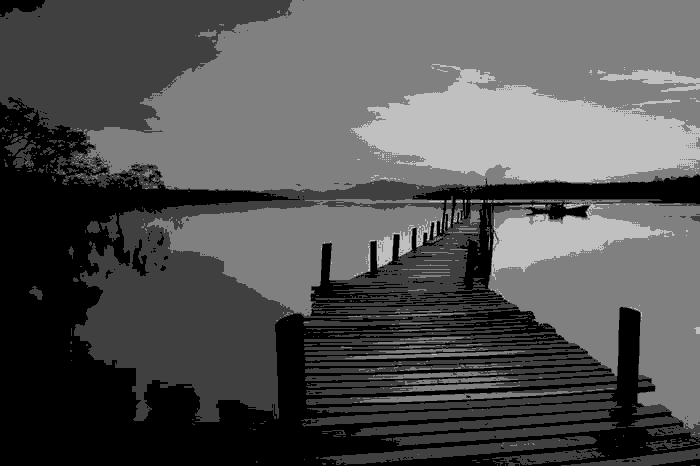
\includegraphics[width=0.4\textwidth]{images/reconstructed_step_2.png} \\
        Step 1: Using Bits [7] & Step 2: Using Bits [7, 6] \\
        \\
        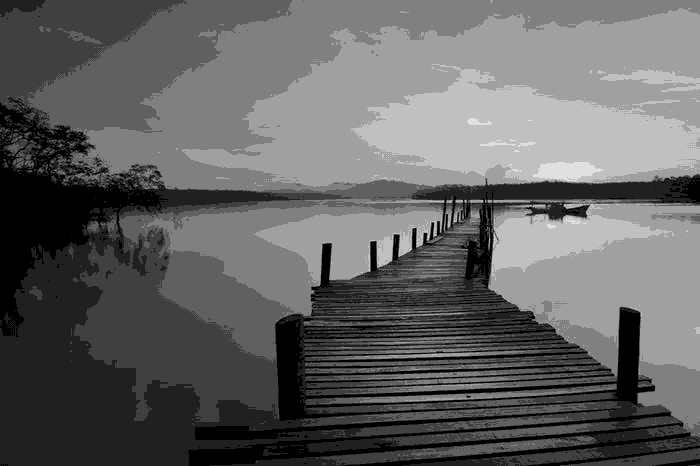
\includegraphics[width=0.4\textwidth]{images/reconstructed_step_3.png} &
        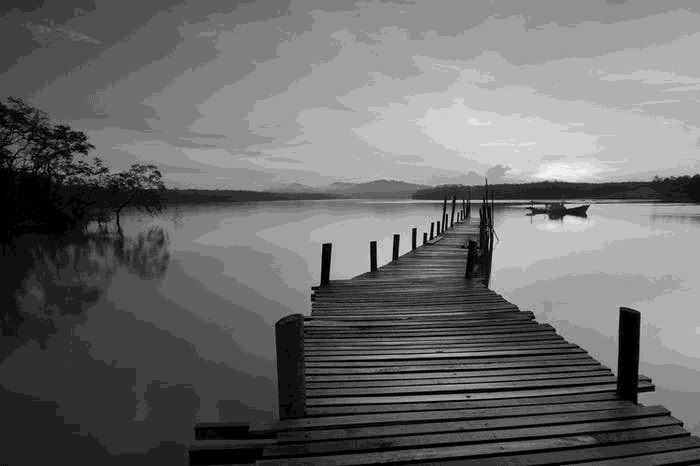
\includegraphics[width=0.4\textwidth]{images/reconstructed_step_4.png} \\
        Step 3: Using Bits [7, 6, 5] & Step 4: Using Bits [7, 6, 5, 4] \\
    \end{tabular}
    \caption{Reconstruction using the 4 most significant bit planes.}
    \label{fig:recon1}
\end{figure}

\begin{figure}[H]
    \centering
    \begin{tabular}{cc}
        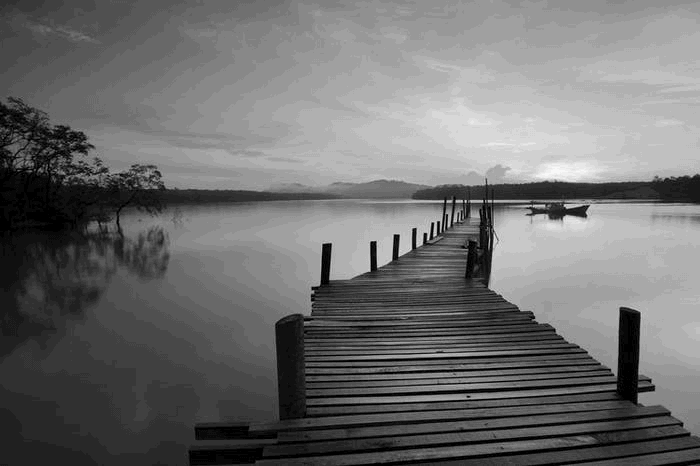
\includegraphics[width=0.4\textwidth]{images/reconstructed_step_5.png} &
        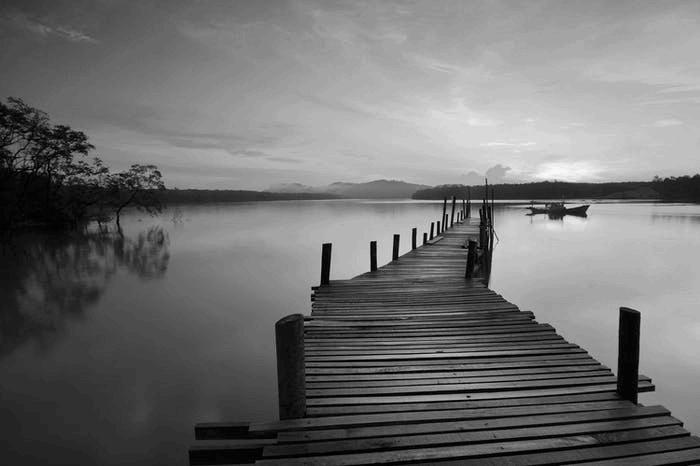
\includegraphics[width=0.4\textwidth]{images/reconstructed_step_6.png} \\
        Step 5: Using Bits [7..3] & Step 6: Using Bits [7..2] \\
        \\
        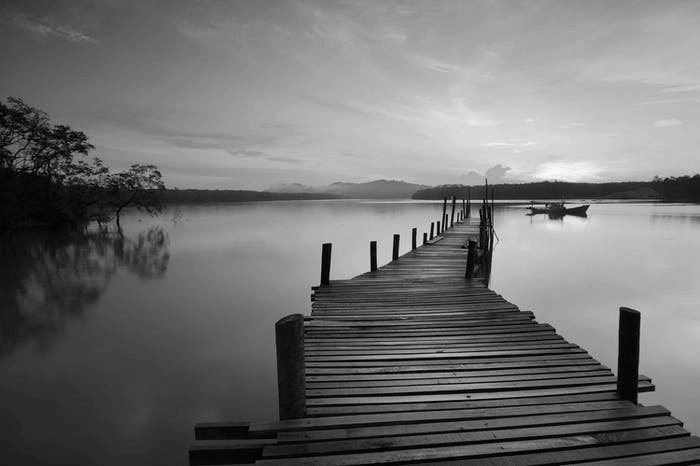
\includegraphics[width=0.4\textwidth]{images/reconstructed_step_7.png} &
        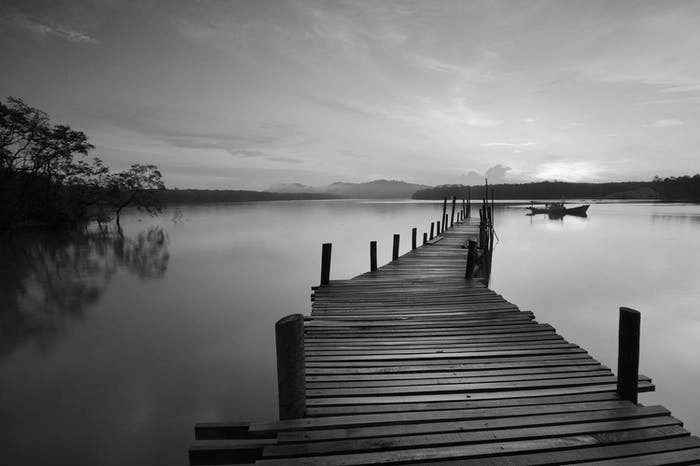
\includegraphics[width=0.4\textwidth]{images/reconstructed_step_8.png} \\
        Step 7: Using Bits [7..1] & Step 8: Using All Bits [7..0] \\
    \end{tabular}
    \caption{Reconstruction using the 4 least significant bit planes, completing the image.}
    \label{fig:recon2}
\end{figure}

\clearpage
\subsection{Observations}
\begin{itemize}
    \item \textbf{MSB Dominance:} The image reconstructed from only the MSB plane (Bit 7) already provides a recognizable, albeit coarse, version of the original image. This demonstrates that the highest bit carries the most significant structural information.
    \item \textbf{Quality Improvement:} As we add subsequent bit planes (6, 5, and 4), the image quality improves dramatically. The reconstruction using the four most significant bits is very close to the original.
    \item \textbf{Fine Details in LSBs:} The lower bit planes (3, 2, 1, and 0) contribute progressively finer details, textures, and subtle variations in shading. The LSB plane (Bit 0) often appears random or noisy, and its contribution to the final image is visually minimal.
    \item \textbf{Video Demonstration:} The generated video file, `bit_plane_progression.mp4`, clearly illustrates this gradual enhancement, with each frame introducing a new bit plane and visibly improving the image quality.
\end{itemize}

% --- Section 4: Conclusion ---
\section{Conclusion}
This assignment successfully demonstrated the bit-plane slicing technique. By decomposing an image into its fundamental bit planes and reconstructing it progressively, we can observe the hierarchical contribution of each bit to the final image. The higher-order bits define the main structure, while the lower-order bits add detail and nuance. This principle is fundamental to various image processing applications, especially lossy image compression, where discarding the lower-bit planes can significantly reduce file size with minimal perceptual loss.

\end{document}